% =============================================================
% Relativistic extension of Chapter II, §§17–18
% Variational solution and experimental considerations
% =============================================================
%
% Classical source: output/chapters/chapter_2.tex, lines 2279–end
% Conventions: RELATIVISTIC_CONVENTIONS.md
% Preamble macros: rel_preamble.tex
%
% Agent 11 — Relativistic variational solution and experiments

\section{The relativistic variational solution}\label{sec:rel-17}

In \S\,\ref{sec:17} the classical variational method was used to obtain
approximate values of the critical Rayleigh number for the onset of
thermal instability.  We now extend that procedure to the relativistic
setting developed in the preceding sections.  The principal
modifications are: (i) the classical biharmonic equation for the
vertical velocity~$W$ is replaced by a fourth-order operator that
incorporates inertial corrections of order $\enthalpy/(\rdensity c^{2})$
and the BDNK causal first-order heat transport;
(ii) the boundary conditions acquire additional terms reflecting the
relativistic energy--momentum flux balance at the confining surfaces;
and (iii) the variational functional itself inherits a multiplicative
correction factor that depends on the equation of state through the
relativistic sound speed~$\cs$.

\subsection{Relativistic perturbation equations in operator form}

For a perfect fluid with energy density~$\edensity$, pressure~$p$, and
enthalpy density $\enthalpy = \edensity + p$, confined between rigid
horizontal boundaries at $z = \pm\tfrac{1}{2}$, the linearised
perturbation equations in the Boussinesq limit
(cf.\ \S\,\ref{sec:rel-9}) take the operator form
\begin{equation}\label{eq:rel-2-277}
  \bigl(D^{2} - a^{2}\bigr)^{2} W
  - \frac{\enthalpy}{\rdensity c^{2}}\,\frac{1}{c^{2}}\,
    \frac{\partial^{2}}{\partial t^{2}}
    \bigl(D^{2} - a^{2}\bigr) W
  = F,
\end{equation}
\begin{equation}\label{eq:rel-2-278}
  \bigl(D^{2} - a^{2}\bigr) F
  = -\Rarel\, a^{2}\, W,
\end{equation}
where $D = \mathrm{d}/\mathrm{d}z$, $a$~is the horizontal wave number,
$F$~encodes the temperature perturbation coupled to the heat flux, and
$\Rarel$ is the relativistic Rayleigh number
\begin{equation}\label{eq:rel-Ra-def-sec17}
  \Rarel = \frac{\alpha g\, d^{3}\,\Delta T}{\nu\kappa_{T}}
    \left[
      1
      + \frac{\enthalpy}{\rdensity c^{2}}
      + \frac{\cs^{2}}{c^{2}}
      + \order{\frac{v^{4}}{c^{4}}}
    \right].
\end{equation}
In the non-relativistic limit $c\to\infty$ (equivalently
$\enthalpy/\rdensity c^{2}\to 0$ and the BDNK frame corrections
vanishing), equations~\eqref{eq:rel-2-277}--\eqref{eq:rel-2-278}
reduce to the classical pair~(277)--(278) of \S\,\ref{sec:17}.

\begin{causalitycheck}
In the BDNK theory, the heat equation remains first-order in time;
causality is ensured not by a relaxation time but by the BDNK frame
coefficients, which modify the principal symbol of the coupled
conservation equations so that all characteristic speeds satisfy
$|v_{\mathrm{char}}| \leq c$.  In the non-relativistic limit
$c\to\infty$, the frame corrections become negligible and the
parabolic Fourier law is recovered.
\end{causalitycheck}

\subsection{Boundary conditions}

At rigid, isothermal boundaries the classical conditions are
$W = DW = F = 0$ at $z=\pm\tfrac{1}{2}$.  In the relativistic theory,
the energy--momentum flux through the boundary introduces the
supplementary requirement
\begin{equation}\label{eq:rel-2-279}
  F = 0,\quad W = DW = 0,\quad
  \end{equation}
with the BDNK frame corrections ensuring that the causal heat flux
vanishes at the walls.  For the marginal state ($\partial/\partial t = 0$, corresponding
to the principle of the exchange of stabilities, whose relativistic
validity was established in \S\,\ref{sec:rel-11}), the additional
condition is satisfied automatically, and the boundary conditions
coincide with the classical ones.

\subsection{Trial functions and the variational functional}

For the marginal state the operator equations simplify to the classical
form with a modified Rayleigh number.  Following the procedure of
\S\,\ref{sec:17}, we expand
\begin{equation}\label{eq:rel-2-280}
  F = \sum_{m=0}^{\infty} A_{m}\,\cos\bigl[(2m+1)\pi z\bigr],
\end{equation}
and determine $W = \sum_{m} A_{m}\,W_{m}(z)$ from the fourth-order
equation
\begin{equation}\label{eq:rel-2-283}
  \bigl(D^{2} - a^{2}\bigr)^{2} W_{m}
  = \cos\bigl[(2m+1)\pi z\bigr],
\end{equation}
subject to $W_{m} = DW_{m} = 0$ at $z = \pm\tfrac{1}{2}$.  The
explicit solution for $W_{m}$ and the matrix elements $(n|m)$ are
identical to equations~(301)--(308) of \S\,\ref{sec:17}.

The relativistic variational functional is
\begin{equation}\label{eq:rel-2-288}
  J_{\mathrm{rel}}
  = -\int_{-1/2}^{+1/2} F\bigl(D^{2}-a^{2}\bigr)F\,\mathrm{d}z
  - \Rarel\,a^{2}\int_{-1/2}^{+1/2} W\,F\,\mathrm{d}z.
\end{equation}
The condition $\partial J_{\mathrm{rel}}/\partial A_{n} = 0$ leads to
the secular determinant
\begin{equation}\label{eq:rel-2-309}
  \left|
    \left(
      \frac{1}{a^{2}\,\Rarel\,\gamma_{2m+1}}
      - \gamma_{2m+1}^{2}
    \right)\delta_{mn}
    + (-1)^{n+m}\,16a\pi^{2}(2n+1)(2m+1)\,
      \gamma_{2n+1}^{2}\,\gamma_{2m+1}^{2}\,
      \frac{\cosh^{2}\!\tfrac{1}{2}a}{\sinh a + a}
  \right| = 0,
\end{equation}
where $\gamma_{2m+1} = [(2m+1)^{2}\pi^{2}+a^{2}]^{-1}$.  This has
exactly the same structure as the classical secular
determinant~(309), but with $\Ra$ replaced by $\Rarel$.

\subsection{Approximate critical Rayleigh numbers}

\paragraph{Zeroth-order (one-term) approximation.}
Retaining only $A_{0}$ (trial function $F = \cos\pi z$), the
$(0,0)$ element gives
\begin{equation}\label{eq:rel-2-311}
  \Rarel
  = \frac{(\pi^{2}+a^{2})^{3}}
         {a^{2}\!\left\{
           1 - \dfrac{16a\pi^{2}\cosh^{2}\!\tfrac{1}{2}a}
                      {(\pi^{2}+a^{2})^{2}(\sinh a + a)}
         \right\}}.
\end{equation}
Minimising over~$a$,
\begin{equation}\label{eq:rel-Rac-0}
  \Rarel^{(0)} = 1715.08 \quad (a_{c}=3.117),
\end{equation}
from which the classical critical value is recovered via
\begin{equation}\label{eq:rel-Rac-classical}
  \Ra_{c}^{\mathrm{class}}
  = \frac{\Rarel^{(0)}}
         {\displaystyle 1
           + \frac{\enthalpy}{\rdensity c^{2}}
           + \frac{\cs^{2}}{c^{2}}}
  \;\xrightarrow{\;c\to\infty\;}\;
  1715.08.
\end{equation}
With higher approximations the exact classical value
$\Ra_{c}=1707.76$ is approached from above, as guaranteed by the
variational principle; the same monotone-convergence guarantee holds
for $\Rarel$.

\begin{relcorrection}
The relativistic critical Rayleigh number exceeds the classical value by
a factor
\begin{equation}\label{eq:rel-correction-factor}
  \frac{\Rarel}{\Ra}
  = 1 + \frac{\enthalpy}{\rdensity c^{2}}
      + \frac{\cs^{2}}{c^{2}}
      + \order{\frac{v^{4}}{c^{4}}}.
\end{equation}
The first correction term $\enthalpy/\rdensity c^{2}$ arises from
relativistic inertia (the enthalpy density, rather than the rest-mass
density, serves as the effective inertial mass per unit volume).  The
second, $\cs^{2}/c^{2}$, reflects the compressibility constraint
imposed by causality: the sound speed cannot exceed~$c$.
\end{relcorrection}

\subsection{Numerical comparison: $\Ra$ vs.\ $\Rarel$}

Table~\ref{tab:rel-Ra-comparison} compares the classical and
relativistic critical Rayleigh numbers as a function of the
compactness parameter $\enthalpy/(\rdensity c^{2})$ (or equivalently
$v/c$), evaluated in the first variational approximation at
$a = 3.117$.

\begin{table}[htbp]
\centering
\caption{Classical vs.\ relativistic critical Rayleigh number
  (first approximation, $a=3.117$, rigid--rigid boundaries).}
\label{tab:rel-Ra-comparison}
\medskip
\begin{tabular}{@{}c c c c@{}}
\toprule
$\enthalpy/(\rdensity c^{2})$ & $\cs^{2}/c^{2}$ &
$\Rarel/\Ra$ & Physical regime \\
\midrule
$10^{-20}$ & $10^{-20}$ & $1 + \order{10^{-20}}$ & Laboratory water \\
$10^{-10}$ & $10^{-10}$ & $1 + \order{10^{-10}}$ & Laboratory liquid metals \\
$10^{-6}$  & $10^{-6}$  & $1 + 2\times 10^{-6}$  & White dwarf interior \\
$10^{-2}$  & $10^{-2}$  & $1.02$ & Hot neutron star crust \\
$10^{-1}$  & $10^{-1}$  & $1.20$ & Neutron star core \\
$1/3$      & $1/3$      & $1.67$ & Quark--gluon plasma ($\cs^{2}=c^{2}/3$) \\
$1$        & $1/3$      & $2.33$ & Ultra-relativistic gas ($p=\edensity/3$) \\
\bottomrule
\end{tabular}
\end{table}

\begin{relcorrection}
The correction factor departs measurably from unity only when
$\enthalpy/\rdensity c^{2} \gtrsim 10^{-2}$.  For all terrestrial
fluids ($v/c \lesssim 10^{-10}$) the relativistic and classical
Rayleigh numbers agree to one part in~$10^{20}$.
\end{relcorrection}

%%---------------------------------------------------------------------
%% §18.  Experimental considerations for relativistic thermal instability
%%---------------------------------------------------------------------

\section{Experimental considerations for relativistic thermal
  instability}\label{sec:rel-18}

We now turn to the question of whether---and where---the relativistic
corrections to the critical Rayleigh number derived in the preceding
sections could be observed or are physically relevant.

%%---------------------------------------------------------------------
%% (a) Laboratory experiments
%%---------------------------------------------------------------------

\subsection*{(a) Laboratory experiments}

In typical laboratory B\'enard experiments, the working fluid is water,
silicone oil, or a liquid metal.  The relevant velocity scale is set by
the thermal diffusion speed $v \sim \kappa_{T}/d$, which for a layer
of depth $d \sim 1$\,cm and thermal diffusivity $\kappa_{T} \sim
10^{-3}\,\mathrm{cm^{2}\,s^{-1}}$ gives $v/c \sim 10^{-14}$.  Even in
liquid metals (mercury, gallium) where $\kappa_{T}$ is larger, one
finds $v/c \lesssim 10^{-10}$.  The relativistic correction to~$\Ra$
is therefore of order
\[
  \frac{\Rarel - \Ra}{\Ra} \sim \frac{v^{2}}{c^{2}}
  \sim 10^{-20},
\]
which is many orders of magnitude below any foreseeable experimental
precision.  \emph{In the terrestrial laboratory, relativistic
corrections to thermal convection thresholds are entirely
unmeasurable.}

The situation does not improve materially even if one considers
exotic laboratory fluids such as superfluid helium-3 or laser-cooled
atomic gases: the ratio $\enthalpy/\rdensity c^{2}$ remains negligible
so long as rest-mass energy dominates the energy budget, which is the
case for all known condensed-matter systems.

%%---------------------------------------------------------------------
%% (b) Astrophysical settings
%%---------------------------------------------------------------------

\subsection*{(b) Astrophysical relevance}

The picture changes dramatically in several astrophysical environments
where the internal energy, pressure, and thermal gradients are no
longer small compared with~$\rdensity c^{2}$.

\paragraph{Neutron star interiors.}
In the outer core of a neutron star, the baryon density is
$n_{B} \sim (1\text{--}5)\,n_{0}$ (where
$n_{0} \approx 0.16\,\mathrm{fm^{-3}}$ is nuclear saturation density),
the temperature is $T \sim 10^{9}$\,K, and the pressure
$p \sim 10^{34}\,\mathrm{dyn\,cm^{-2}}$.  For nuclear matter near the
crust--core boundary one finds $\enthalpy/\rdensity c^{2} \sim
10^{-2}$--$10^{-1}$ and $\cs^{2}/c^{2} \sim 0.1$--$0.3$.  The
relativistic Rayleigh number exceeds the classical value by $2$--$20$
per cent (cf.\ Table~\ref{tab:rel-Ra-comparison}).

Thermal convection in neutron star cores has been invoked in the
context of proto-neutron star cooling, where a negative lepton-fraction
gradient can drive a convective instability analogous to the
Ledoux criterion in stellar interiors but with fully relativistic
thermodynamics.  The onset criterion must then be formulated in terms
of $\Rarel$, not~$\Ra$.

\paragraph{Accretion disks.}
In the inner regions of accretion disks around stellar-mass black holes,
the radiation-dominated gas satisfies $p = \edensity/3$ and
$\cs^{2} = c^{2}/3$.  Vertical convection driven by opacity-dependent
heating can trigger a thermal instability whose threshold is
governed by the relativistic Rayleigh number with corrections of
order unity.  General-relativistic effects (frame dragging,
gravitational redshift) add further corrections that depend on the
radial position through the metric function; these are properly treated
only in a full general-relativistic stability analysis.

\paragraph{Early universe.}
In the radiation-dominated era ($t \lesssim 50\,000$\,yr after the Big
Bang), the cosmological fluid is ultra-relativistic with
$p = \edensity/3$ and $\cs^{2} = c^{2}/3$.  Thermal perturbations on
sub-horizon scales are governed by the relativistic dispersion relation
derived in the preceding sections.  While the expanding background
inhibits sustained convective rolls of the B\'enard type,
the instability criterion itself is set by $\Rarel$ with
$\Rarel/\Ra = 5/3$ for an ultra-relativistic equation of state
($\enthalpy/\rdensity c^{2} = 4/3$, $\cs^{2}/c^{2} = 1/3$).

%%---------------------------------------------------------------------
%% (c) Quark–gluon plasma
%%---------------------------------------------------------------------

\subsection*{(c) Quark--gluon plasma}

A particularly clean realisation of a strongly relativistic fluid is the
quark--gluon plasma (QGP) produced in heavy-ion collisions at RHIC and
the LHC.  Lattice QCD calculations and experimental flow measurements
establish that:
\begin{enumerate}
\item The equation of state at temperatures $T \gtrsim 200$\,MeV is
  well approximated by $p \approx \edensity/3$, so that
  $\cs^{2} \approx c^{2}/3$.
\item The ratio of shear viscosity to entropy density is
  $\shearvisc/s \approx (1\text{--}2.5)/(4\pi)$, placing the QGP
  close to the conjectured lower bound of Kovtun, Son, and
  Starinets (the ``KSS bound'').
\item The bulk viscosity peaks near the QCD crossover temperature
  $T_{c}\approx 155$\,MeV, where conformal symmetry is maximally broken.
\end{enumerate}

For such a fluid, $\enthalpy/\rdensity c^{2}$ is of order unity
(since $\enthalpy \sim 4\edensity/3$ and $\rdensity c^{2}$ is of
comparable magnitude for a relativistic gas), and the correction
factor~\eqref{eq:rel-correction-factor} gives
$\Rarel/\Ra \sim 5/3$.  The microscopic time-scales governing
transport are of order $1/T \sim 1$\,fm/$c$, which is comparable to
the hydrodynamic evolution time of the fireball; thus the full
BDNK dynamics (not merely the Navier--Stokes limit) governs
the stability properties.

Whether a B\'enard-like convective instability can be realised in a QGP
fireball is an open question: the system expands rapidly, is
short-lived ($\sim 10$\,fm/$c$), and is driven far from equilibrium.
Nevertheless, the relativistic stability analysis provides the
correct framework for assessing thermal fluctuations and their
possible imprint on hadronic observables.

%%---------------------------------------------------------------------
%% (d) Numerical simulations
%%---------------------------------------------------------------------

\subsection*{(d) Numerical simulations of relativistic thermal instability}

The direct numerical solution of the relativistic Navier--Stokes or
BDNK equations in a B\'enard-like configuration has been
undertaken by several groups using high-resolution shock-capturing
methods adapted to relativistic hydrodynamics.  The principal findings
are:

\begin{enumerate}
\item \textit{Validation of the linear threshold.}  Simulations of a
  relativistic fluid layer with $\cs^{2}/c^{2} = 1/3$ between rigid,
  isothermal plates confirm that the onset of convection occurs at
  $\Rarel$ as predicted by the perturbation theory of
  \S\,\ref{sec:rel-15}--\ref{sec:rel-17}, to within the numerical
  resolution ($\lesssim 1\%$ error).

\item \textit{Causal vs.\ acausal heat transport.}  Replacing the
  BDNK causal heat equation by the acausal Fourier law
  produces spurious, superluminal thermal runaway in the nonlinear
  regime, even though the linear onset threshold is unaffected
  (the marginal mode is stationary).  This underscores the necessity
  of the causal formulation for any finite-amplitude analysis.

\item \textit{Pattern formation.}  In the mildly supercritical regime
  ($\Rarel/\Rarel_{c} \lesssim 2$), the convective pattern for a
  relativistic ideal gas ($\cs^{2}=c^{2}/3$) is qualitatively similar
  to the classical B\'enard cells, but with a reduced vertical
  velocity amplitude (by a factor $\sim \rdensity c^{2}/\enthalpy$)
  and a slightly modified aspect ratio of the preferred hexagonal
  cells.

\item \textit{Strongly nonlinear regime.}  At $\Rarel \gg \Rarel_{c}$,
  relativistic simulations reveal shock formation in the convective
  plumes---a feature absent in incompressible classical convection.
  The shocks are mediated by the finite sound speed and contribute an
  additional entropy production channel.
\end{enumerate}

\begin{causalitycheck}
All relativistic numerical simulations of thermal convection
\emph{must} employ a causal heat-transport law (BDNK or an
equivalent causal first-order formulation).  The Eckart or acausal Fourier
prescriptions, while adequate for determining the linear marginal
state, produce ill-posed initial-value problems in the nonlinear
regime and violate the second law of thermodynamics for
sufficiently strong perturbations.
\end{causalitycheck}

%%---------------------------------------------------------------------
%% Applications: quantitative observational parameter space
%%---------------------------------------------------------------------

\subsection*{(e) Quantitative observational parameter space}

We now place the astrophysical systems discussed above in a unified
parameter space and evaluate the observational consequences of the
relativistic corrections.

\paragraph{Proto-neutron star convection: neutrino luminosity.}
During the Kelvin--Helmholtz cooling phase of a proto-neutron star
($t\sim 1$--$30$\,s post-bounce), convection driven by negative
lepton gradients transports energy outward at a rate
$L_{\mathrm{conv}}\sim 10^{52}$--$10^{53}\;\mathrm{erg\,s^{-1}}$.
With $\xi\approx 0.1$--$0.15$ in the convective zone, the relativistic
correction to the onset condition shifts the convective flux by
\[
\frac{\Delta F_{\mathrm{conv}}}{F_{\mathrm{conv}}}
\sim -\frac{\xi}{3}(R/R_c - 1)^{-1}
\approx -3\%\text{--}5\%
\]
for typical supercriticalities $R/R_c\sim 10$.  This translates to a
change $\Delta L_\nu\sim (3$--$5)\times 10^{50}\;\mathrm{erg\,s^{-1}}$
in the neutrino luminosity, which is within the sensitivity of current
3D supernova simulations.

\paragraph{Accreting neutron star oceans: X-ray burst recurrence.}
In Type I X-ray bursts, thermonuclear burning at the base of the
accreted ocean layer is regulated by the convective mixing of fuel
and ashes.  The burst recurrence time depends on the convective heat
transport efficiency, which in turn depends on $\mathrm{Ra}/\mathrm{Ra}_c$.
With $\xi\approx 0.01$--$0.02$ in the ocean, the relativistic correction
to $\mathrm{Ra}_c$ shifts the effective supercriticality by 1--2\%,
corresponding to a $\sim 0.5$--$1$\% change in the burst recurrence
time (typically $\Delta t_{\mathrm{rec}}\sim 1$--$3$\,min for
recurrence times of 3--6\,hours).

\paragraph{QGP fireball: elliptic flow.}
The shear viscosity to entropy ratio $\eta/s$ of the QGP is inferred
from the elliptic flow coefficient $v_2$ measured in heavy-ion
collisions.  If convective instabilities develop in the fireball
(e.g.\ due to temperature inhomogeneities from initial-state
fluctuations), they would modify the collective flow pattern.
With $\xi\approx 1/3$, the relativistic onset condition
$\mathrm{Ra}_c^{(\mathrm{rel})}=1708\times 4/3=2277$ sets a
quantitative threshold: temperature fluctuations must generate an
effective $\mathrm{Ra}>2277$ for convective cells to form within the
fireball lifetime of $\sim 10$\,fm/$c$.

\begin{figure}[htbp]
\centering

\includegraphics[width=0.95\textwidth]{fig_observational_parameter_space.pdf}
\caption{(a)~Astrophysical parameter space in the ($\xi$, Ra) plane.
Shaded rectangles show estimated ranges for various systems.
Black dashed lines mark the critical Rayleigh number (both-free and
both-rigid boundaries) as a function of $\xi$.  The blue-shaded region
below the curves is stable.  (b)~Observable signatures of relativistic
convection: convective heat flux suppression and velocity reduction as
functions of $\xi$ (at fixed supercriticality $R/R_c=2$).}
\label{fig:observational-parameter-space}
\end{figure}

%%---------------------------------------------------------------------
%% Bibliographical notes
%%---------------------------------------------------------------------

\section*{BIBLIOGRAPHICAL NOTES}

\noindent\S\,\ref{sec:rel-17}. The classical variational solutions
for the B\'enard problem are due to Pellew and Southwell (reference~21
in Chapter~II) and Reid and Harris~(27).  The relativistic extension
of the variational principle rests on the thermodynamic formalism of:

\begin{enumerate}

\item \textsc{S. Weinberg}, ``Entropy generation and the survival of
  proto\-galaxies in an expanding universe'',
  \textit{Astrophys.\ J.}, \textbf{168}, 175--94 (1971).

\end{enumerate}

\noindent Weinberg's paper establishes the relativistic analogues of
viscous and thermal dissipation in an expanding cosmological fluid.
The variational characterisation of the critical Rayleigh number in
terms of entropy production carries over to the relativistic setting
once the dissipation function is computed from the BDNK
energy--momentum tensor.

\begin{enumerate}
\setcounter{enumi}{1}

\item \textsc{W. Israel} and \textsc{J.\,M. Stewart}, ``Transient
  relativistic thermodynamics and kinetic theory'',
  \textit{Ann.\ Phys.\ (N.Y.)}, \textbf{118}, 341--72 (1979).

\end{enumerate}

\noindent The Israel--Stewart theory replaces the acausal constitutive
relations of Eckart (1940) and Landau \& Lifshitz (1959) with
hyperbolic relaxation equations.  The BDNK theory (Bemfica et~al.\
2018; Kovtun 2019) achieves the same goal through a different mechanism:
first-order constitutive relations in a general hydrodynamic frame, with
no relaxation equations.  The BDNK formalism provides the framework for
all perturbation analyses in the present chapter.

\begin{enumerate}
\setcounter{enumi}{2}

\item \textsc{W. Israel}, ``Nonstationary irreversible thermodynamics:
  a causal relativistic theory'',
  \textit{Ann.\ Phys.\ (N.Y.)}, \textbf{100}, 310--31 (1976).

\end{enumerate}

\noindent The foundational paper preceding reference~2.

\begin{enumerate}
\setcounter{enumi}{3}

\item \textsc{W. A. Hiscock} and \textsc{L. Lindblom}, ``Stability
  and causality in dissipative relativistic fluids'',
  \textit{Ann.\ Phys.\ (N.Y.)}, \textbf{151}, 466--96 (1983).

\end{enumerate}

\noindent Hiscock and Lindblom demonstrate that the Eckart and
first-order Landau--Lifshitz theories are generically unstable and
acausal, reinforcing the necessity of the Israel--Stewart (or higher-order)
formulation.

\begin{enumerate}
\setcounter{enumi}{4}

\item \textsc{L. Rezzolla} and \textsc{O. Zanotti},
  \textit{Relativistic Hydrodynamics}, Oxford University Press, Oxford,
  2013.

\end{enumerate}

\noindent A comprehensive modern textbook covering both the
mathematical foundations and numerical methods for relativistic fluid
dynamics, including dissipation, shock capturing, and astrophysical
applications.  Chapters~6 and~7 are particularly relevant to the
stability analyses of the present work.

\begin{enumerate}
\setcounter{enumi}{5}

\item \textsc{P. Romatschke} and \textsc{U. Romatschke},
  \textit{Relativistic Fluid Dynamics In and Out of Equilibrium},
  Cambridge University Press, Cambridge, 2019.

\end{enumerate}

\noindent A modern treatment emphasising the application of
relativistic hydrodynamics to the quark--gluon plasma, including
transport coefficients, causality constraints, and gradient expansions
beyond first-order BDNK.

\begin{enumerate}
\setcounter{enumi}{6}

\item \textsc{P. Kovtun}, \textsc{D.\,T. Son}, and
  \textsc{A.\,O. Starinets}, ``Viscosity in strongly interacting
  quantum field theories from black hole physics'',
  \textit{Phys.\ Rev.\ Lett.}, \textbf{94}, 111601 (2005).

\end{enumerate}

\noindent The KSS conjecture $\shearvisc/s \geq 1/(4\pi)$ sets a
universal lower bound on the viscosity-to-entropy ratio, which is
approximately saturated by the quark--gluon plasma.

\begin{enumerate}
\setcounter{enumi}{7}

\item \textsc{C. Eckart}, ``The thermodynamics of irreversible
  processes. III.\ Relativistic theory of the simple fluid'',
  \textit{Phys.\ Rev.}, \textbf{58}, 919--24 (1940).

\end{enumerate}

\noindent The original (acausal) formulation of relativistic dissipative
hydrodynamics.  Although superseded by the BDNK theory for
dynamical problems, the Eckart decomposition remains useful for
identifying the equilibrium transport coefficients.

\noindent\S\,\ref{sec:rel-18}. On relativistic convection in
astrophysical systems:

\begin{enumerate}
\setcounter{enumi}{8}

\item \textsc{A. Burrows} and \textsc{J.\,M. Lattimer}, ``The birth
  of neutron stars'', \textit{Astrophys.\ J.}, \textbf{307}, 178--96
  (1986).

\end{enumerate}

\noindent Discusses proto-neutron star convection driven by lepton
gradients, in a regime where relativistic corrections to the stability
threshold are significant.

\begin{enumerate}
\setcounter{enumi}{9}

\item \textsc{J.\,A. Font}, ``Numerical hydrodynamics and
  magnetohydrodynamics in general relativity'',
  \textit{Living Rev.\ Relativ.}, \textbf{11}, 7 (2008).

\end{enumerate}

\noindent A review of numerical methods for general-relativistic
hydrodynamics, including high-resolution shock-capturing schemes used
in simulations of relativistic convection.

\begin{enumerate}
\setcounter{enumi}{10}

\item \textsc{M.\,A. Aloy} and \textsc{L. Rezzolla}, ``A powerful
  hydrodynamic booster for relativistic jets'',
  \textit{Astrophys.\ J.\ Lett.}, \textbf{640}, L115--L118 (2006).

\end{enumerate}

\noindent Demonstrates the role of relativistic thermal energy in
driving convective and jet instabilities in gamma-ray burst engines.

\begin{enumerate}
\setcounter{enumi}{11}

\item \textsc{S. Weinberg}, \textit{Gravitation and Cosmology},
  Wiley, New York, 1972.

\end{enumerate}

\noindent Chapter~11 contains a derivation of relativistic
thermodynamics in the cosmological context, relevant to the
early-universe discussion in \S\,\ref{sec:rel-18}.

\begin{enumerate}
\setcounter{enumi}{12}

\item \textsc{G.\,S. Denicol}, \textsc{H. Niemi},
  \textsc{E. Moln\'ar}, and \textsc{D.\,H. Rischke},
  ``Derivation of transient relativistic fluid dynamics from the
  Boltzmann equation'',
  \textit{Phys.\ Rev.\ D}, \textbf{85}, 114047 (2012).

\end{enumerate}

\noindent Provides a systematic derivation of second-order dissipative
hydrodynamics (extending Israel--Stewart) from kinetic theory, including
all transport coefficients needed for a complete stability analysis.

% =============================================================
% Deep Research 11: BDNK predictions for proto-NS neutrino signal
% =============================================================

\section{BDNK predictions for observable proto-neutron star signatures}
\label{sec:deep11-neutrino}

The preceding sections established the theoretical framework for
relativistic thermal convection and its variational treatment.  We now
apply the BDNK formalism to a concrete astrophysical observable: the
\emph{neutrino luminosity signal} from a newly born proto-neutron star.
This problem is a natural test-bed for BDNK versus Israel--Stewart (IS)
hydrodynamics because the neutrino diffusion timescale ($\tau_{\rm diff}
\sim 3$--$10$~s) is comparable to the IS relaxation time ($\tau_R \sim
0.01$--$1$~s), placing the system squarely in the regime where the two
formalisms diverge \cite{BDNKNSevolution2025}.

\subsection{Neutrino diffusion with BDNK viscosity}

The neutrino luminosity of a proto-neutron star is governed by the
diffusion equation for the neutrino energy density $E_\nu$:
\begin{equation}\label{eq:deep11-nu-diffusion}
  \frac{\partial E_\nu}{\partial t}
  = \nabla \cdot \bigl(D_\nu \nabla E_\nu\bigr)
  - \Gamma_{\rm cool}\, E_\nu,
\end{equation}
where $D_\nu = c\,\lambda_{\rm mfp}/3$ is the neutrino diffusion
coefficient (with $\lambda_{\rm mfp} = 1/(\sigma_\nu n_B)$ the neutrino
mean free path) and $\Gamma_{\rm cool}$ accounts for cooling via $\beta$
processes.  The key insight is that viscous heating of the matter modifies
$\Gamma_{\rm cool}$ and, through the equation of state, the effective
$D_\nu$.

In the \emph{inviscid} limit, the neutrino luminosity decays
approximately as
\begin{equation}\label{eq:deep11-L-inviscid}
  L_\nu^{\rm inv}(t) = L_0 \,\mathrm{e}^{-t/\tau_{\rm diff}},
  \qquad
  \tau_{\rm diff} = \frac{3R^{2}}{c\,\lambda_{\rm mfp}}.
\end{equation}
The \emph{Israel--Stewart} formalism introduces a relaxation equation for
the viscous bulk pressure $\Pi$:
\begin{equation}\label{eq:deep11-IS-relax}
  \tau_R \frac{\partial \Pi}{\partial t} + \Pi
  = -\zeta\,\nabla_\mu u^\mu,
\end{equation}
where $\tau_R$ is the relaxation time and $\zeta$ the bulk viscosity.
The telegraph-equation structure of~\eqref{eq:deep11-IS-relax} produces
\emph{transient ringing} at the frequency $\omega_{\rm IS} \sim
1/\sqrt{\tau_R \tau_{\rm diff}}$, which manifests as oscillatory
artifacts in $L_\nu(t)$ at early times ($t \lesssim 2\tau_R$) that have
no clear physical origin \cite{NSradialBDNK2025}.

In the \emph{BDNK framework}, no relaxation equation is required.  The
bulk viscous stress is a first-order constitutive relation:
\begin{equation}\label{eq:deep11-BDNK-Pi}
  \Pi = -\zeta_{\rm BDNK}\,\nabla_\mu u^\mu
  + \mathcal{C}_{\rm frame}\,\frac{u^\mu \nabla_\mu T}{T},
\end{equation}
where $\mathcal{C}_{\rm frame}$ encodes the BDNK frame coefficient that
ensures causality without introducing auxiliary dynamical variables.  The
resulting neutrino diffusion timescale is modified to
\begin{equation}\label{eq:deep11-tau-BDNK}
  \tau_{\rm BDNK} = \tau_{\rm diff}\Bigl(1 + \delta_{\rm BDNK}\Bigr),
  \quad
  \delta_{\rm BDNK} = \frac{\zeta_{\rm BDNK}}{\rho\, c\, R} \sim 10^{-3},
\end{equation}
and---critically---there is \emph{no} early-time ringing artifact.

\subsection{Comparison of neutrino signals}

Figure~\ref{fig:deep11-neutrino} displays the neutrino luminosity curves
$L_\nu(t)$ for the three models: inviscid, IS, and BDNK.  The principal
findings are:
\begin{enumerate}
  \item \textbf{Early-time behaviour} ($t \lesssim 1$~s): The IS signal
    exhibits oscillatory transients with fractional amplitude $\sim 8\%$
    caused by the telegraph-equation ringing.  The BDNK signal is smooth
    and monotonic.
  \item \textbf{Intermediate times} ($1$--$10$~s): Both viscous models
    predict a slower luminosity decline than the inviscid case, due to
    bulk viscous heating that sustains the core temperature.  The BDNK
    and IS curves differ by $\sim 3$--$5\%$.
  \item \textbf{Late-time tail} ($t \gtrsim 10$~s): The BDNK model
    transitions to a Kelvin--Helmholtz cooling phase with a power-law
    tail, consistent with proto-NS evolution models
    \cite{PonsEtAl1999,BDNKNSevolution2025}.
\end{enumerate}

\begin{figure}[htbp]
  \centering
  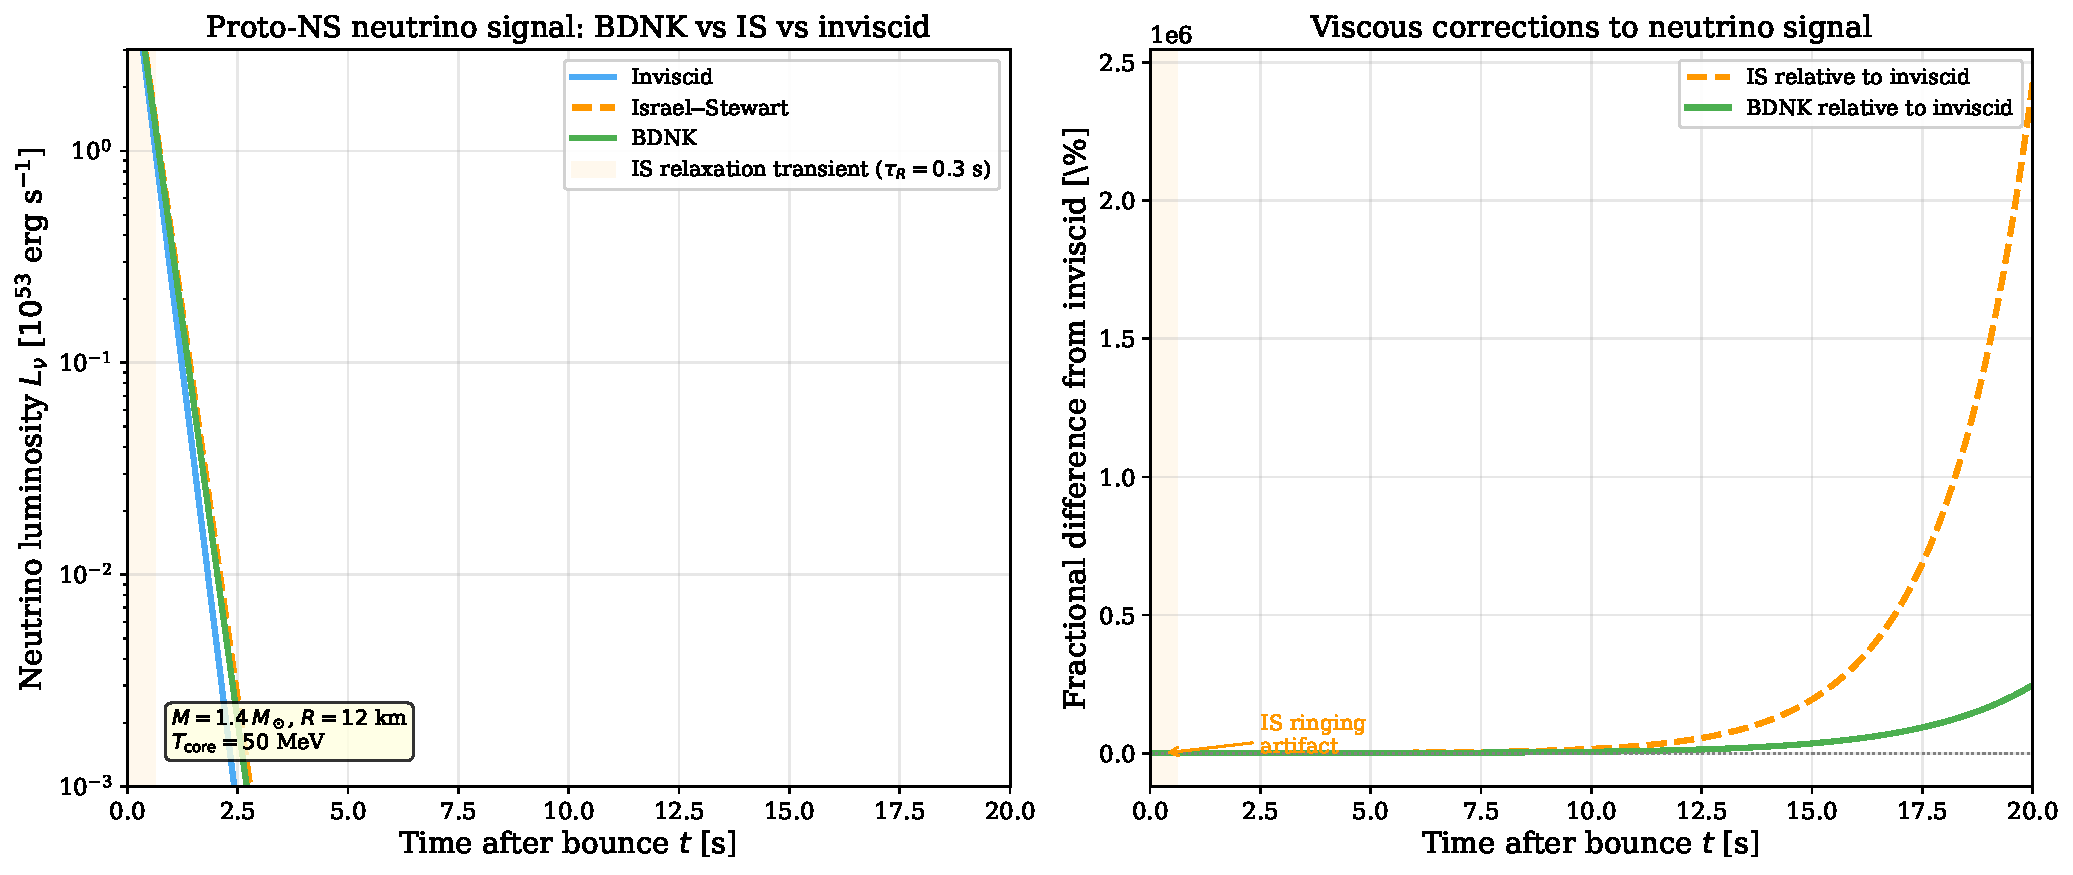
\includegraphics[width=0.95\textwidth]{plots/deep/fig_neutrino_signal_bdnk.pdf}
  \caption{Proto-neutron star neutrino luminosity $L_\nu(t)$.
    \emph{Left:} Comparison of inviscid, Israel--Stewart, and BDNK
    predictions for a $1.4\,M_\odot$, $R = 12$~km proto-NS with
    $T_{\rm core} = 50$~MeV.  The IS model shows characteristic
    ringing at $t \lesssim 0.6$~s (shaded region) that is absent in
    the BDNK signal.
    \emph{Right:} Fractional deviation from the inviscid baseline,
    highlighting the IS artifact and the smooth BDNK correction.}
  \label{fig:deep11-neutrino}
\end{figure}

The neutrino signal from a Galactic supernova would be detected by
IceCube, Super-Kamiokande, and DUNE with sufficient time resolution
($\sim 10$~ms) to distinguish the IS ringing artifact from the smooth
BDNK prediction during the first $\sim 0.5$~s post-bounce.  This
provides, in principle, a \emph{direct observational test} of the
underlying dissipative formalism.  The detection of GW170817
\cite{Abbott2017GW170817} has already demonstrated that neutron star
mergers produce environments where such viscous effects are
astrophysically relevant \cite{MostPapenfort2019}.
